\section{Profunctors / Grothendieck construction}
\label{sec:org7dd09e1}
There are two possible ways to define a relation $R$ between two sets $A,B$:
\begin{enumtag}{r}
\item \label{r_1} a relation $R$ is a subset of the cartesian product $A\times B$;
\item \label{r_2} a relation $R$ is a function $A\times B \to \{0,1\}$.
\end{enumtag}
Note that the notion of `relation between $A$ and $B$' is inherently symmetric, in the sense that such $R$ can be regarded both as a relation `from' $A$ `to' $B$, and as a relation `from' $B$ `to' $A$.

Furthermore, every relation $R$ between sets $A,B$ gives rise to a \emph{Galois connection} 
\[R^* :PA^\op \leftrightarrows PB : R_* \label{adjunzia} \]
between the powersets $PA=2^A$ and $PB = 2^B$: the set $U\subset A$ goes to the set $R^*U$ of all $b$ such that $(a,b)\in R$ for all $a\in U$; in an exactly symmetric way, a set $V\subseteq B$ goes to the set 
\[R_*V = \{a\in A\mid (a,b) \in R,\, \forall b\in V\}.\]
Unwinding the definition, it is asy to see that $R^* \dashv R_*$.

From here, using a process known as `categorification' \cite{baez_catego}, we can replace a two-valued relation $R\subseteq A\times B$ with a \emph{set-valued} functor $\clA^\op\times\clB \to \Set$ between two (small) categories $\clA,\clB$.\footnote{The reason why the category $\clA$ is twisted with an `$^\op$' functor is that we want to bestow the hom functor $\hom_{\clA} : \clA^\op\times\clA \to \Set$ with the r\^ole of identity arrow; in the categorification perspective, hom plays the r\^ole of the diagonal relation $R=\Delta : A\to A\times A$.} More precisely, we can give the following definition.
\begin{definition}[Profunctor]\label{def_profu}
  
\end{definition}
The intuition behind \autoref{def_profu} is that $\fkR(A,B)$ is the \emph{type} whose terms are all proofs che tra $(A,B)\in\clA^\op\times\clB$ sussiste la `relazione generalizzata' $\fkR$. This intuition agrees with the fact that when instead of $\Set$ a profunctor $\fkR$ takes values in the 0-dimensional category $\{0\le 1\}$, then the type of proofs that $R(A,B)$ is a yes/no kind of space.

From here, one can build a rich and expressive theory; we are contempt with a careful analysis of the analogue of \ref{r_2} and \eqref{adjunzia} above: the latter is the scope of \autoref{sec:org1a423df}, we now concentrate on describing an ubiquitary technical tool in category theory.
\subsection{Grothendieck construction}
The Grothendieck construction is the tool allowing to formalise the equivalence between a relation understood as a function $R : A\times B \to \{0,1\}$, and a subset $R\subseteq A\times B$, when `relation' is understood in the sense of \autoref{def_profu} above, i.e. a profunctor $\fkR : \clA \pto \clB$. Each such $\fkR$ can be realised as a suitable `fibration' $p_\fkR : \clE \to \clA^\op\times\clB$, that in turn uniquely determines $\fkR$.
We now recall a few basic definitions.
\begin{definition}\label{eltsf}
	Let $\clC$ be an ordinary category, and let $W : \clC\to \Set$ be a functor; the \emph{category of elements} $\elts{\clC}{W}$ of $W$ is the category which results from the pullback
  \[
    \xymatrix{
      \elts{\clC}{W}\ar[r]\ar[d] \pb & \Set_* \ar[d]^U \\
      \clC \ar[r]_W & \Set
    }
  \]
  where $U : \Set_*\to\Set$ is the forgetful functor which sends a pointed set to its underlying set.
  
  More explicitly, $\elts{\clC}{W}$ has objects the pairs $(C\in\clC, u\in WC)$, and morphisms $(C,u)\to (C',v)$ those $f\in \clC(C,C')$ such that $W(f)(u)=v$.
\end{definition}
\begin{definition}[Discrete fibration]
	\label{def:dfib}
	A \emph{discrete fibration} of categories is a functor $G : \clE \to \clC$ with the property that for every object $E\in\clE$ and every arrow $p : C\to GE$ in $\clC$ there is a unique $q : E'\to E$ `over $p$', i.e. such that $Gq=p$.
\end{definition}
Taking as morphisms between discrete fibrations the morphisms in $\Qat/\clC$, we can define the category $\DFib(\clC)$ of discrete fibrations \emph{over} $\clC$.
\begin{proposition}\label{fibelem}
	The category of elements $\elts{\clC}{W}$ of a functor $W : \clC\to \Set$ comes equipped with a canonical \emph{discrete fibration} to the domain of $W$, which we denote $\Sigma : \elts{\clC}{W}\to \clC$, defined forgetting the distinguished element $u\in Wc$.
\end{proposition}
With this terminology at hand, we can consider the \emph{category of elements} \ref{eltsf} of a functor $F : \clC\to \Set$; this sets up a functor from $\Qat(\clC,\Set)$ to the category of discrete fibrations over $\clC$: the Grothendieck construction asserts that this is an equivalence of categories.%, as defined in \ref{def:equcat}.
\begin{theorem}\label{thm:equconfib}
	There is an equivalence of categories
	\[
		\Qat(\clC^\op,\Set) \to \DFib(\clC)
	\]
	defined by the correspondence sending $F\in\Qat(\clC,\Set)$ to its \emph{fibration of elements}  $\Sigma_F : \elts{\clC}{F} \to \clC$.
\end{theorem}
The inverse correspondence sends a discrete fibration $\Phi : \clE \to \clC$ to the functor whose action on objects and morphisms is depicted in the following image:
\begin{center}
  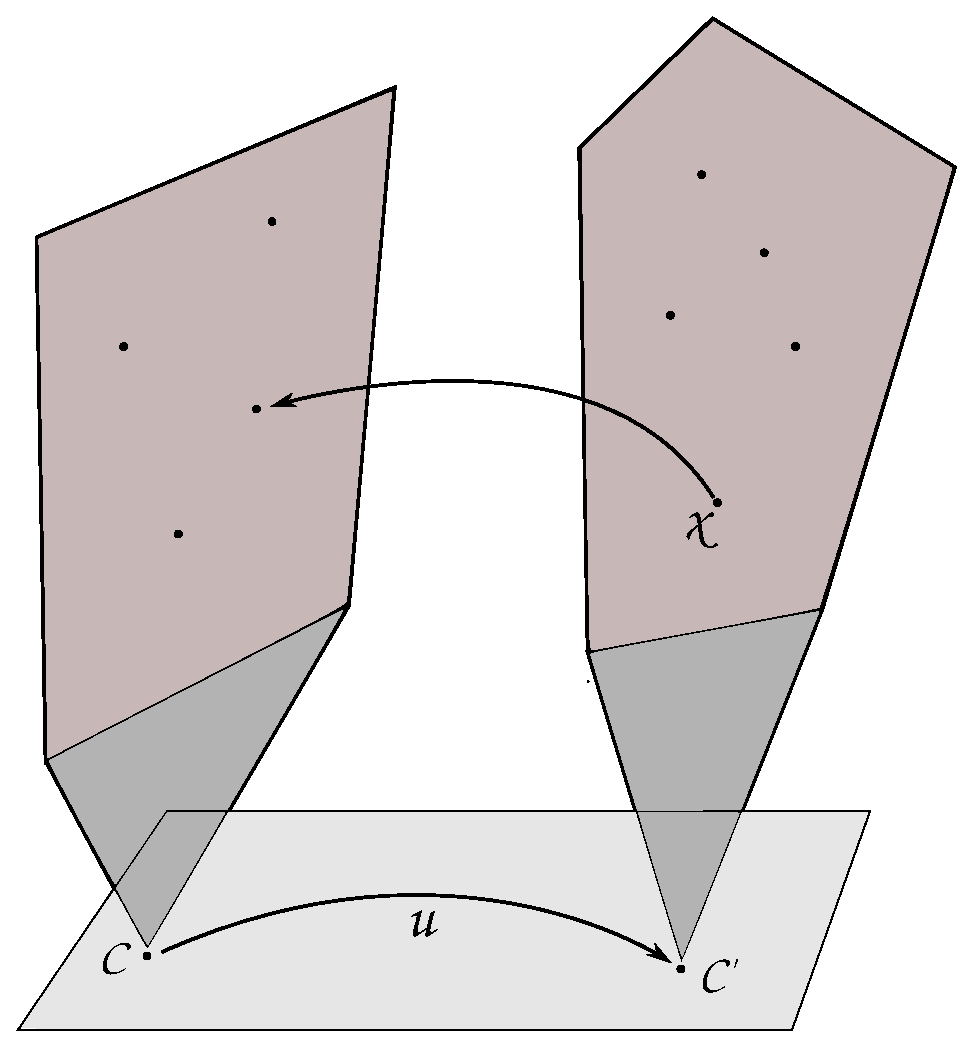
\includegraphics[width=.325\textwidth]{disegno.eps}
\end{center}
\begin{corollary}
  Given a profunctor $\fkR : \clA \pto \clB$, regarded as a functor $R : \clA^\op\times \clB \to \Set$, we can consider the category of elements $\elts{\clA^\op\times\clB}{R}$; this is often called the \emph{collage} or the \emph{graph} of $R$.
\end{corollary}
